% F5 — The object-and-action model (Palantir's four-part language: data · logic · action ·
% security) as it exists in this campaign. Objects = what we write to disk (typed; schemas exist
% since 2026-09-02 for the ones marked \ensuremath{\blacklozenge}); links = solid when a declared field carries them
% (trigger key, sha256, commit), dashed when they exist only by naming convention; actions =
% labelled arrows, solid when first-class on disk (identity-stamped, receipted), dashed when
% PROPOSED; roles = the bottom band. Census 2026-09-02. Every box maps to rows of Table T1.
% COLOUR GRAMMAR (PI 2026-09-03): object colour = who WRITES it: blue = written by code (products, receipts, audits,
% action events, the derived burst state); amber = carries a human identity (approval stamps); white = law and
% documents (register row, lesson, commit pin, the burst catalog row). Roles band: human amber, agent green, hook and
% script blue.
\documentclass[tikz,border=4pt]{standalone}
\usepackage[T1]{fontenc}
\usepackage{lmodern}
\usepackage{amssymb}
\usetikzlibrary{positioning,calc,shapes.geometric,arrows.meta,fit,backgrounds}
\newcommand{\nohyph}{\hyphenpenalty=10000 \exhyphenpenalty=10000 }
\definecolor{codefill}{RGB}{219,231,245}\definecolor{codeline}{RGB}{59,110,165}
\definecolor{agentfill}{RGB}{226,240,217}\definecolor{agentline}{RGB}{58,125,52}
\definecolor{humanfill}{RGB}{253,236,200}\definecolor{humanline}{RGB}{191,124,0}
\definecolor{docline}{RGB}{110,110,110}
\begin{document}
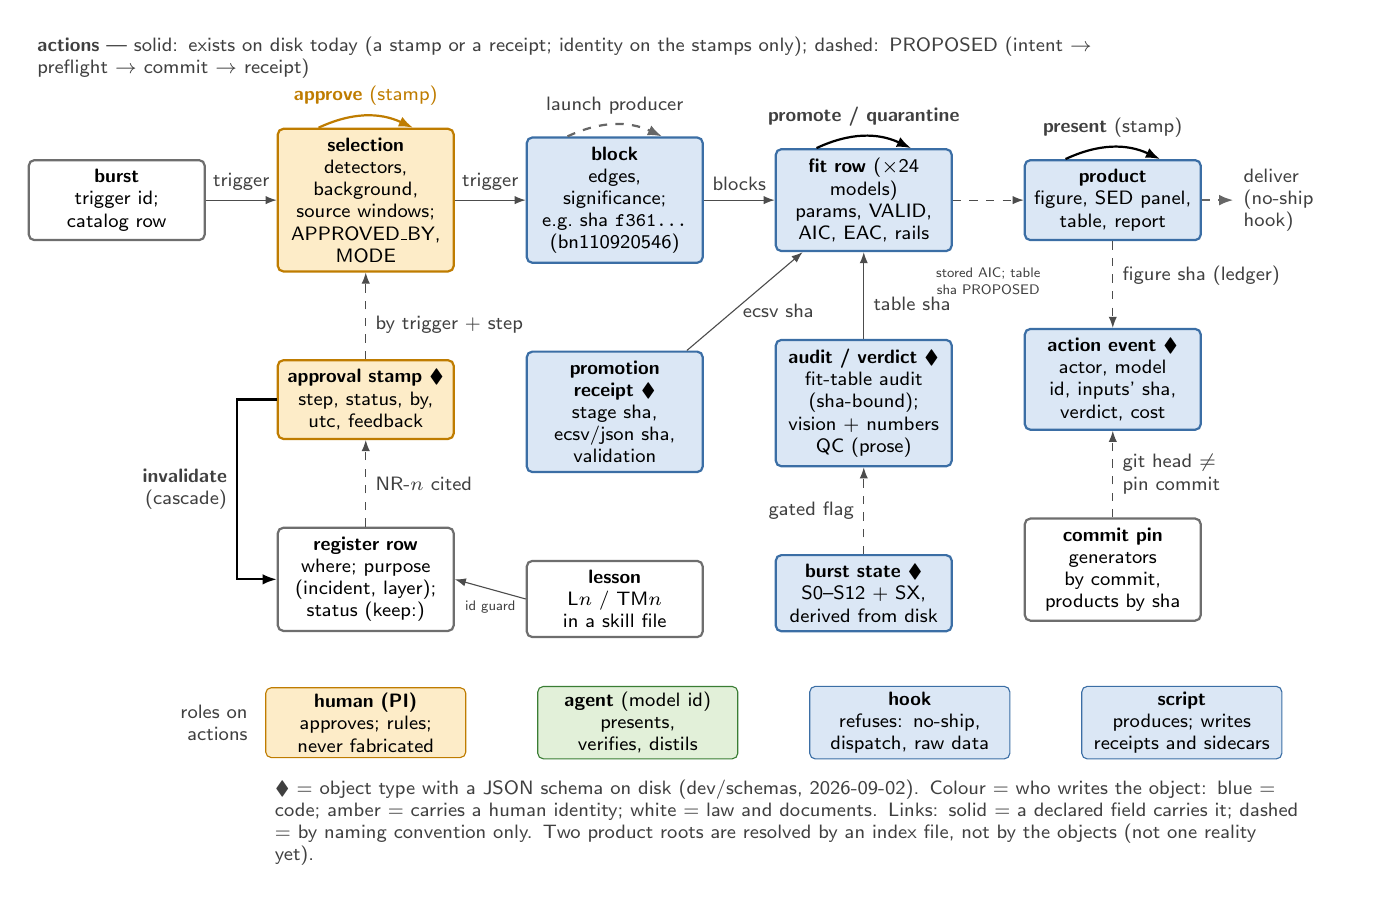
\begin{tikzpicture}[
  font=\sffamily\scriptsize, node distance=3mm and 9mm,
  obj/.style={draw=docline, thick, rounded corners=2pt, fill=white, text width=20mm, align=center, minimum height=9mm, execute at begin node=\nohyph},
  objc/.style={obj, fill=codefill, draw=codeline},
  objh/.style={obj, fill=humanfill, draw=humanline},
  act/.style={-{Latex[length=1.8mm]}, thick},
  actp/.style={act, dashed, black!60},
  acth/.style={act, humanline},
  link/.style={-{Latex[length=1.4mm]}, thin, black!70},
  linkc/.style={link, dashed},
  lab/.style={font=\sffamily\scriptsize, text=black!75, execute at begin node=\nohyph},
  role/.style={draw=docline, rounded corners=2pt, text width=24mm, align=center, font=\sffamily\scriptsize, inner sep=2pt, execute at begin node=\nohyph},
  roleh/.style={role, fill=humanfill, draw=humanline}, rolea/.style={role, fill=agentfill, draw=agentline}, rolec/.style={role, fill=codefill, draw=codeline}]

% ---- objects (row 1: the burst's chain of products) ----
\node[obj] (burst) {\textbf{burst}\\trigger id; catalog row};
\node[objh, right=of burst] (sel) {\textbf{selection}\\detectors, background, source windows; APPROVED\_BY, MODE};
\node[objc, right=of sel] (blk) {\textbf{block}\\edges, significance; e.g.\ sha \texttt{f361\ldots} (bn110920546)};
\node[objc, right=of blk] (fit) {\textbf{fit row} ($\times$24 models)\\params, VALID, AIC, EAC, rails};
\node[objc, right=of fit] (prod) {\textbf{product}\\figure, SED panel, table, report};

% ---- row 2: the records about the products ----
\node[objh, below=11mm of sel] (stamp) {\textbf{approval stamp} \ensuremath{\blacklozenge}\\step, status, by, utc, feedback};
\node[objc, below=11mm of blk] (receipt) {\textbf{promotion receipt} \ensuremath{\blacklozenge}\\stage sha, ecsv/json sha, validation};
\node[objc, below=11mm of fit] (audit) {\textbf{audit / verdict} \ensuremath{\blacklozenge}\\fit-table audit (sha-bound); vision + numbers QC (prose)};
\node[objc, below=11mm of prod] (trace) {\textbf{action event} \ensuremath{\blacklozenge}\\actor, model id, inputs' sha, verdict, cost};

% ---- row 3: the law ----
\node[obj, below=11mm of stamp] (reg) {\textbf{register row}\\where; purpose (incident, layer); status (keep:)};
\node[obj, below=11mm of receipt] (lesson) {\textbf{lesson}\\L$n$ / TM$n$ in a skill file};
\node[objc, below=11mm of audit] (state) {\textbf{burst state} \ensuremath{\blacklozenge}\\S0--S12 + SX, derived from disk};
\node[obj, below=11mm of trace] (pin) {\textbf{commit pin}\\generators by commit, products by sha};

% ---- declared links (solid) and links by convention (dashed) ----
\draw[link] (burst) -- node[lab, above] {trigger} (sel);
\draw[link] (sel) -- node[lab, above] {trigger} (blk);
\draw[link] (blk) -- node[lab, above] {blocks} (fit);
\draw[linkc] (fit) -- (prod);
\node[lab, anchor=north, text width=16mm, align=center, font=\sffamily\tiny] at ($(fit.south east)!0.5!(prod.south west)+(0,-1.5mm)$) {stored AIC; table sha PROPOSED};
\draw[link] (receipt) -- node[lab, right, pos=0.4] {ecsv sha} (fit);
\draw[link] (audit) -- node[lab, right, pos=0.4] {table sha} (fit);
\draw[linkc] (stamp.north) -- node[lab, right, pos=0.4] {by trigger + step} (sel.south);
\draw[linkc] (prod.south) -- node[lab, right, pos=0.4] {figure sha (ledger)} (trace.north);
\draw[linkc] (state.north) -- node[lab, left, pos=0.5] {gated flag} (audit.south);
\draw[linkc] (pin.north) -- node[lab, right, pos=0.5, text width=14mm] {git head $\neq$ pin commit} (trace.south);
\draw[linkc] (reg.north) -- node[lab, right, pos=0.5] {NR-$n$ cited} (stamp.south);
\draw[link] (lesson.west) -- node[lab, below=0.3mm, font=\sffamily\tiny] {id guard} (reg.east);

% ---- actions: first-class on disk (solid), proposed (dashed) ----
\node[lab, above=9mm of burst.north west, anchor=south west, text width=140mm, align=left] {\textbf{actions} --- solid: exists on disk today (a stamp or a receipt; identity on the stamps only); dashed: PROPOSED (intent $\to$ preflight $\to$ commit $\to$ receipt)};
\draw[acth] ($(sel.north)+(-6mm,0)$) to[bend left=25] node[lab, above, text=humanline] {\textbf{approve} (stamp)} ($(sel.north)+(6mm,0)$);
\draw[act] ($(fit.north)+(-6mm,0)$) to[bend left=25] node[lab, above] {\textbf{promote / quarantine}} ($(fit.north)+(6mm,0)$);
\draw[act] ($(prod.north)+(-6mm,0)$) to[bend left=25] node[lab, above] {\textbf{present} (stamp)} ($(prod.north)+(6mm,0)$);
\draw[act] (stamp.west) -- ++(-5mm,0) |- node[lab, left, pos=0.25, text width=12mm, align=right] {\textbf{invalidate} (cascade)} (reg.west);
\draw[actp] ($(blk.north)+(-6mm,0)$) to[bend left=25] node[lab, above] {launch producer} ($(blk.north)+(6mm,0)$);
\draw[actp] (prod.east) -- ++(4mm,0) node[lab, right, text width=12mm, align=left] {deliver (no-ship hook)};

% ---- roles band ----
\node[roleh, below=7mm of reg] (rh) {\textbf{human (PI)}\\approves; rules; never fabricated};
\node[rolea, right=of rh] (ra) {\textbf{agent} (model id)\\presents, verifies, distils};
\node[rolec, right=of ra] (rk) {\textbf{hook}\\refuses: no-ship, dispatch, raw data};
\node[rolec, right=of rk] (rs) {\textbf{script}\\produces; writes receipts and sidecars};
\node[lab, left=1mm of rh.west, anchor=east, text width=14mm, align=right] {roles on actions};

% legend
\node[lab, below=1.5mm of rh.south west, anchor=north west, text width=130mm, align=left] {\ensuremath{\blacklozenge} = object type with a JSON schema on disk (dev/schemas, 2026-09-02). Colour = who writes the object: blue = code; amber = carries a human identity; white = law and documents. Links: solid = a declared field carries it; dashed = by naming convention only. Two product roots are resolved by an index file, not by the objects (not one reality yet).};
\end{tikzpicture}
\end{document}
